\documentclass[border=8pt]{standalone}
\usepackage{fontspec}
\setmainfont{TeX Gyre Heros}
\setsansfont{TeX Gyre Heros}
\usepackage{tikz}
\usetikzlibrary{arrows.meta,positioning,shapes.geometric,shapes.misc,shapes.symbols,fit,backgrounds,calc,chains}
\definecolor{ink}{HTML}{111827}
\definecolor{band}{HTML}{F3F4F6}
\definecolor{band2}{HTML}{E5E7EB}
\definecolor{accent}{HTML}{1D4ED8}
\definecolor{accentlight}{HTML}{DBEAFE}
\definecolor{warn}{HTML}{B91C1C}
\definecolor{warnlight}{HTML}{FEE2E2}
\definecolor{ok}{HTML}{047857}
\definecolor{oklight}{HTML}{D1FAE5}
\tikzset{
  >={Stealth[length=2.6mm]},
  box/.style={draw=ink, line width=0.6pt, rounded corners=9pt, fill=white, align=center,
              inner sep=4pt, font=\small},
  pill/.style={box, rounded corners=13pt},
  key/.style={box, fill=accentlight, draw=accent, line width=0.9pt},
  soft/.style={box, fill=band},
  dec/.style={draw=ink, line width=0.6pt, diamond, aspect=2.2, align=center, inner sep=1.5pt,
              font=\footnotesize, fill=white},
  arr/.style={->, draw=ink, line width=0.6pt},
  darr/.style={->, draw=ink, line width=0.6pt, dashed},
  lbl/.style={font=\footnotesize, fill=white, inner sep=1.5pt},
  layer/.style={draw=band2, fill=band, rounded corners=6pt},
  title/.style={font=\bfseries\small, align=left, anchor=west},
}
\begin{document}
\sffamily\hyphenpenalty=10000\exhyphenpenalty=10000

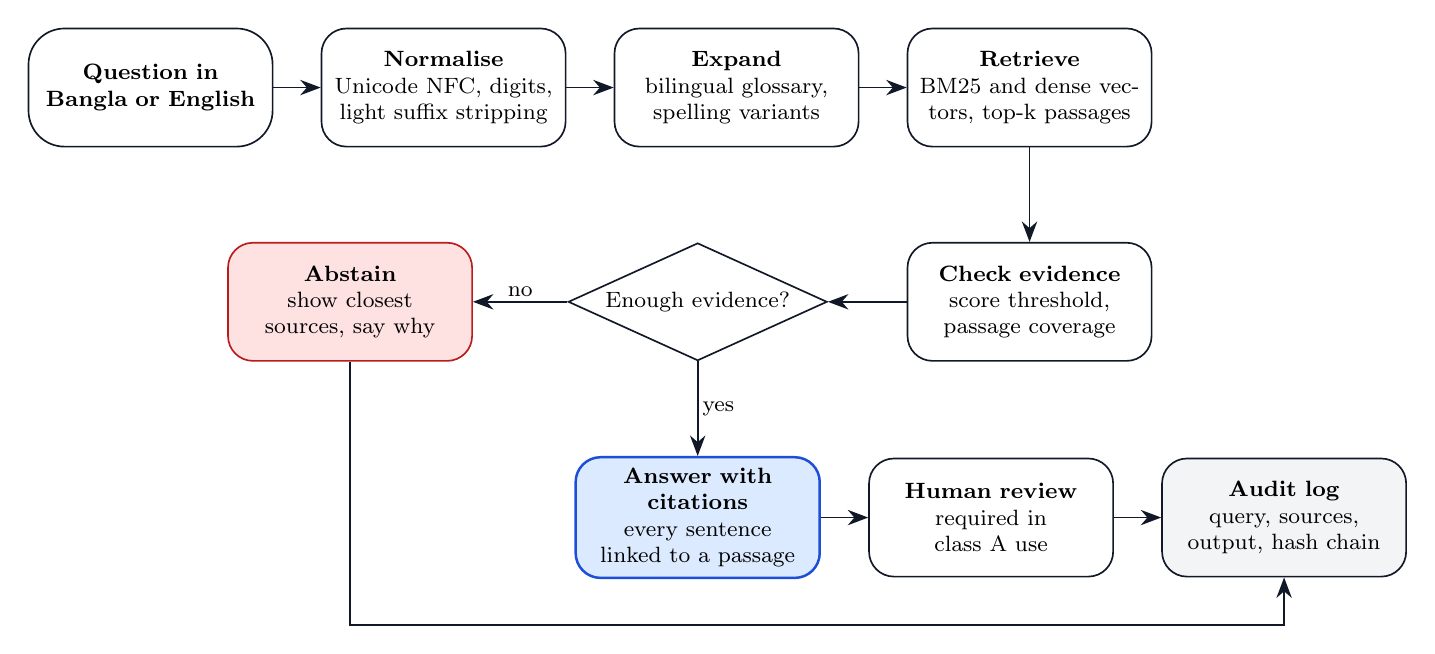
\begin{tikzpicture}[node distance=6mm and 6mm]
\tikzset{st/.style={box, minimum width=31mm, minimum height=15mm, font=\footnotesize, text width=28mm}}
\node[pill, minimum width=31mm, minimum height=15mm, font=\footnotesize, text width=28mm] (q) {\textbf{Question in Bangla or English}};
\node[st, right=of q] (n) {\textbf{Normalise}\\Unicode NFC, digits, light suffix stripping};
\node[st, right=of n] (e) {\textbf{Expand}\\bilingual glossary, spelling variants};
\node[st, right=of e] (r) {\textbf{Retrieve}\\BM25 and dense vectors, top-k passages};
\node[st, below=12mm of r] (k) {\textbf{Check evidence}\\score threshold, passage coverage};
\node[dec, left=10mm of k, text width=24mm] (d) {Enough evidence?};
\node[key, minimum width=31mm, minimum height=15mm, font=\footnotesize, text width=28mm, below=12mm of d] (a) {\textbf{Answer with citations}\\every sentence linked to a passage};
\node[box, draw=warn, fill=warnlight, minimum width=31mm, minimum height=15mm, font=\footnotesize, text width=28mm, left=12mm of d] (x) {\textbf{Abstain}\\show closest sources, say why};
\node[st, right=of a] (h) {\textbf{Human review}\\required in class A use};
\node[soft, minimum width=31mm, minimum height=15mm, font=\footnotesize, text width=28mm, right=of h] (l) {\textbf{Audit log}\\query, sources, output, hash chain};
\draw[arr] (q) -- (n); \draw[arr] (n) -- (e); \draw[arr] (e) -- (r); \draw[arr] (r) -- (k);
\draw[arr] (k) -- (d);
\draw[arr] (d) -- node[lbl, right]{yes} (a);
\draw[arr] (d) -- node[lbl, above]{no} (x);
\draw[arr] (a) -- (h); \draw[arr] (h) -- (l);
\draw[arr] (x.south) |- ($(l.south)+(0,-6mm)$) -- (l.south);
\end{tikzpicture}
\end{document}
